\documentclass[11pt]{article}

\usepackage{geometry}
\geometry{a4paper}

\usepackage{graphicx}
\usepackage{amssymb}
\usepackage{physics}
\usepackage{amsmath}
\usepackage{lipsum}
\usepackage[shortlabels]{enumitem}

\usepackage{cite} %Uses proper indexing when citing multiple papers
\usepackage{authblk} %Shows all authors with e-mail addresses and affiliations properly on the page

%%%%%%%%%%%%%%%%%%%%%%%%%%%%%%% INFO %%%%%%%%%%%%%%%%%%%%%%%%%%%%%%%%%%%%%%%%%
\title{Extensive Study of the Wobbling Properties in $^{163}$Lu for the Positive and Negative Parity States} 

\author[1,2]{Robert Poenaru \thanks{E-mail: robert.poenaru@drd.unibuc.ro}}
\author[2,3]{Apolodor Aristotel Raduta \thanks{E-mail: raduta@nipne.ro}}

\affil[1]{Doctoral School of Physics, University of Bucharest, Romania}
\affil[2]{\textit{Horia Hulubei} National Institute for Physics and Nuclear Engineering, M\u{a}gurele-Bucharest, Romania}
\affil[3]{Academy of Romanian Scientists, Bucharest, Romania}
%%%%%%%%%%%%%%%%%%%%%%%%%%%%%%% INFO %%%%%%%%%%%%%%%%%%%%%%%%%%%%%%%%%%%%%%%%%

\date{\today}

\begin{document}

\bibliographystyle{unsrt}

\maketitle

%%%%%%%%%%%%%%%%%%%%%%%%%%%%%%% TEXT %%%%%%%%%%%%%%%%%%%%%%%%%%%%%%%%%%%%%%%%%
\begin{abstract}
A new interpretation on the wobbling structure in $^{163}$Lu is developed, based on the concept of parity symmetry. It is known that four wobbling bands are experimentally observed in this isotope, where three of them are considered as wobbling phonon excitations (namely $TSD_2$, $TSD_3$, and $TSD_4$) and the yrast band for the ground state (that is TSD1). In the present work, the trial function that is used for obtaining the wobbling spectrum is analyzed in terms of its behavior under the rotation operation. Indeed, due to a specific symmetry to rotations with $\pi$ around the 2-axis of the triaxial system, the parity becomes a good quantum number. As such, the trial function admits solutions with negative parity, which belong to the rotational states in $TSD_4$. A unified description of all the triaxial super-deformed bands in $^{163}$Lu is achieved with the new formalism.
\end{abstract}

\section{Introduction}

Triaxiality in nuclei has become an interesting topic for physicists over the years, mainly due to its great challenge of measure it experimentally, but also for its large number of characteristics that are said to be resulting from these kind of shapes. Moreover, stable triaxial shapes are of rare occurrence across the chart of nuclides \cite{moller2006global}, since the predominant character of nuclei is either spherical or axially symmetric. Over the last two decades, it has been shown that triaxiality plays a crucial role in measurements of important quantities like proton emission probabilities \cite{delion2006theories}, separation energies of the nucleons \cite{moller2006global}, and also fission barriers in heavy nuclei  \cite{moller2009heavy}, however, concrete evidences of triaxiality in nuclei were still missing or under investigation. A tremendous work was given in finding a clear signature for non-axially symmetric shapes: effects such as anomalous signature splitting \cite{hamamoto1988triaxial}, signature inversion \cite{bengtsson1984signature}, and staggering of $\gamma$ bands \cite{stachel1982triaxiality} were pointed, but only recently two clear fingerprints of nuclear triaxiality have emerged in the literature, based on both experimental and theoretical findings. Indeed, the phenomena of \emph{chiral symmetry breaking} and that of \emph{wobbling motion} (W.M.) are considered as unique characteristics of nuclear triaxiality. 

Chirality consists in the existence of a pair of chiral twin bands with an identical structure and almost similar energies. These bands are expected to appear due to the coupling of valence nucleons and the collective mode of rotation that could drive the total spin away from any of the three principal planes, giving rise to both left-handed and right-handed orientation of the angular momentum vectors \cite{frauendorf1997tilted}. A rigorous investigation of all the nuclei with chiral bands is given by Xiong and Wang in \cite{xiong2019nuclear}, where reportedly a total of 59 chiral doublet bands in 47 such nuclei are confirmed. As a matter of fact, 8 of these nuclei have multiple chiral doublets. 

On the other hand, the experimental observations regarding wobbling motion have been quite rare, even though this kind of collective motion has been theoretically predicted almost 50 years ago by Bohr and Mottelson \cite{bohr1998nuclear} when they were investigating the rotational modes of a triaxial nucleus by means of a Triaxial Rotor Model (TRM). Therein, they showed that for a triaxial rotor, the main rotational motion is around the axis with the largest moment of inertia (MOI), as it is energetically the most favorable. This mode is quantum mechanically disturbed by the rotation around the other two axes, since rotation around any of the three principal axes of the system are possible, due to the anisotropy of the three different MOIs (that is $\mathcal{I}_1\neq\mathcal{I}_2\neq\mathcal{I}_3$).

W.M. can be viewed as the quantum analogue to the motion of the asymmetric top, whose rotation around the axis with largest MOI is energetically favored and stable. A uniform rotation about this axis will have the lowest energy for a given angular momentum (spin). As the energy increases, this axis will start to precess with a harmonic type of oscillation about the space-fixed angular momentum vector, giving rise to a family of wobbling bands, each characterized by a wobbling phonon number $n_w$. The resulting quantal spectrum will be a sequence of rotational $\Delta I=2$ bands, with alternating signature number for each wobbling excitation. According to \cite{bohr1998nuclear}, it is possible to obtain the wobbling spectrum of any triaxial rigid rotor, by using the information related to its angular momentum $I$, moments of inertia $\mathcal{I}_{1,2,3}$, rotational frequency $\omega_\text{rot}$, wobbling frequency $\omega_\text{wob}$ as follows:

\begin{align}
    E_\text{rot}=\sum_i\left(\frac{\hbar^2}{2\mathcal{I}_k}\right)I^2_k\approx\frac{\hbar^2}{2\mathcal{I}_1}I(I+1)+\hbar\omega_\text{wob}\left(n_w+\frac{1}{2}\right)\ , \label{wobbling_eq}
\end{align}

with $\omega_\text{wob}$ given by the following expression:
\begin{align}
    \hbar\omega_\text{wob}=\hbar\omega_\text{rot}\sqrt{\frac{(\mathcal{I}_1-\mathcal{I}_2)(\mathcal{I}_1-\mathcal{I}_3)}{\mathcal{I}_2\mathcal{I}_3}}\ .
\end{align}

where the rotational frequency of the rigid rotor is given by $\hbar\omega_\text{rot}=\frac{\hbar I^2}{\mathcal{I}_1}$. In Eq. \ref{wobbling_eq}, the approximation of very large MOI along 1-axis is considered (i.e., $\mathcal{I}_1>>\mathcal{I}_2,\mathcal{I}_3$), and $I(I+1)=I_1^2+I_2^2+I_3^2$. One can see that the wobbling motion is expressed as a 1-dimensional vibration with only one variable, since the energy of the zero-point fluctuation is $\frac{\hbar\omega_\text{wob}}{2}$ \cite{hagemann2003quantized}.

Just for an illustrative purpose, Figure \ref{simple-wobbling-family} shows a theoretical spectrum for the wobbling bands within a triaxial rigid rotor. The family of wobbling bands are obtained from a set of three moments of inertia (along the three principal axes), a given angular momentum, and different wobbling phonon numbers. Moreover, in Figure \ref{simple-wobbling-family}, the tilting of the angular momentum away from the rotational axis is sketched, where the tilt increases with the increase in the wobbling excitation. In a given sequence of wobbling bands, both the intra-band $\Delta I=2$ as well as inter-band $\Delta I=1$ transitions have a strong $E2$ collective character.

\begin{figure}
\centering
\begin{minipage}{.6\textwidth}
  \centering
  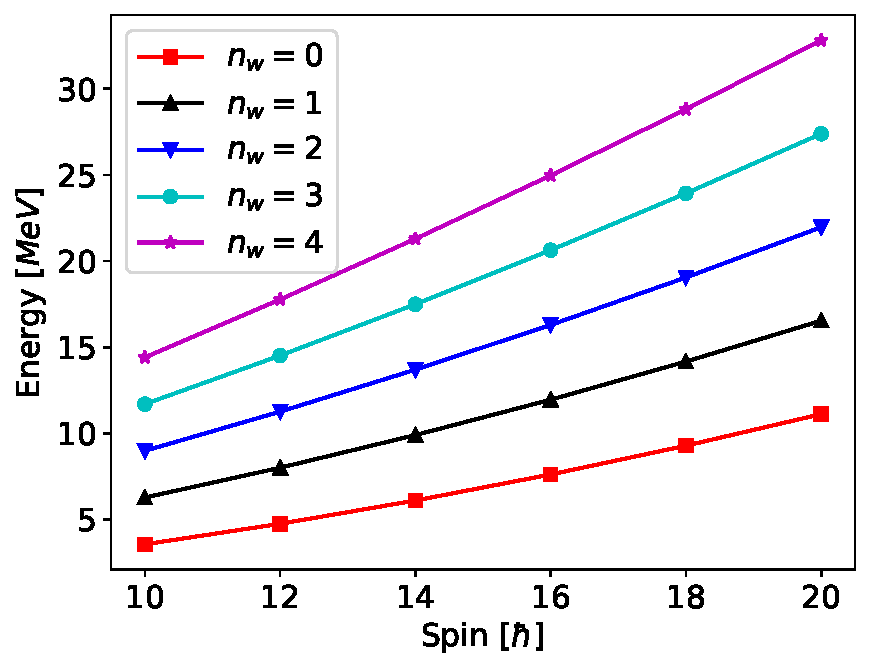
\includegraphics[width=1\linewidth]{figs/simple_wobbling_spectrum.pdf}
  %  \caption{A family of wobbling bands for a triaxial rigid rotor (schematic representation). The calculations were done for $\mathcal{I}_1:\mathcal{I}_2:\mathcal{I}_3=25:5:2$.}
    % \label{simple-wobbling-family}
\end{minipage}%
\begin{minipage}{.4\textwidth}
  \centering
 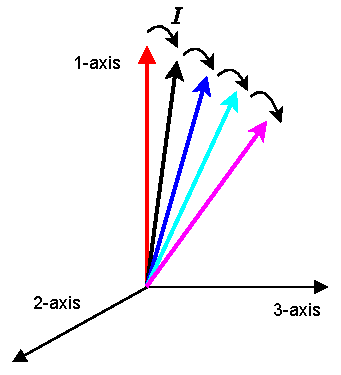
\includegraphics[width=0.8\linewidth]{figs/wobbling_tilting_axis.pdf}
   % \caption{Tilting of the angular momentum away from the rotational axis, with increase in the wobbling phonon excitation.}
    % \label{wobbling-tilt}
\end{minipage}
\label{simple-wobbling-family}
\caption{Family of wobbling bands for a simple triaxial rotor (left-side). Tilting of the angular momentum vector away from the rotational axis (right-side). This schematic representation was done for an arbitrary set of MOIs $\mathcal{I}_1:\mathcal{I}_2:\mathcal{I}_3=25:5:2$.}
\end{figure}

It is important to mention that the wobbling spectrum described by Eq. \ref{wobbling_eq} and graphically represented in Figure \ref{simple-wobbling-family} was firstly predicted for an even-even triaxial nucleus \cite{bohr1998nuclear}. This predicted wobbling mode has not been experimentally confirmed yet. However, the first experimental evidence for wobbling excitations in nuclei was for an even-odd nucleus, namely $^{163}$Lu, where a single one-phonon wobbling band was measured initially \cite{odegaard2001evidence}, followed by two additional wobbling bands discovered one year later \cite{jensen2002evidence,jensen2002wobbling}.

After the first discovery of wobbling bands in $^{163}$Lu ($Z=71$), an entire series of even-odd isotopes with $A\approx160$ were experimentally confirmed as \emph{wobblers}: $^{161}$Lu, $^{165}$Lu, $^{167}$Lu, and $^{167}$Ta. In these nuclei, the wobbling mode appears due to the coupling of a valence nucleon (the so-called $\pi(i_{13/2})$ intruder) to a triaxial core, driving the entire nuclear system up to large deformation ($\epsilon\approx0.4$) \cite{schnack1995superdeformed}.

With time, several nuclei in which WM occurs were also reported in regions of smaller $A$. Indeed, two isotopes with $A\approx130$: $^{133}$La \cite{biswas2019longitudinal} and $^{135}$Pr \cite{matta2017transverse,sensharma2019two} were identified as having wobbling bands, which emerged from the coupling with a triaxial even-even core of another intruder (the $\pi(h_{11/2})$ nucleon) for $^{135}$Pr, and an additional pair of positive parity quasi-protons which are making an alignment with the short axis of the triaxial rotor for $^{105}$Pr. The resulting coupling in both cases have a deformation $\epsilon=0.16$ \cite{matta2017transverse,biswas2019longitudinal}, which is obviously smaller than the deformation in the heavier nuclei within the $A\approx160$ region. A third nucleus that also lies in this mass region was confirmed very recently by Chakraborty et. al. in \cite{chakraborty2020multiphonon}, namely the odd-$A$ $^{127}$Xe, where a total of four wobbling bands have been reported by the team (two yrast bands, and two excited phonon bands with $n_w=1$ and $n_w=2$).

Some additional progress towards a more comprehensive wobbling spectroscopy was made in the $A\approx100$ mass region, with an experimental evidence for $^{105}$Pd that showed of two such bands that are built on a $\nu(h_{11/2})$ configuration, the first one so far in which a valence neutron couples to the triaxial core \cite{timar2019experimental}. The resulting configuration drives the nuclear system up to deformation $\epsilon\approx0.26$.

The heaviest nuclei known so far in which WM has been experimentally observed are the isotopes $Z=79$ with $A=183$ \cite{nandi2020first} and $A=187$ \cite{sensharma2020longitudinal}, respectively. However, for the case of $^{187}$Au, there is an ongoing debate \cite{guo2020risk} whether the two wobbling bands ($n_w=0$ and $n_w=1$) are bands with wobbling character, or if they are of magnetic nature (which would exclude the wobbling phonon interpretation).

Regarding the wobbling motion for the even-even nuclei (behavior that was described above through the schematic representation from Figure \ref{simple-wobbling-family}), the experimental results are very fragmentary, with unclear evidence on such collective behavior in nuclei. However, some embryos of even-even wobblers have been reported in the recent years. For example, the $^{112}$Ru ($Z=44$) nucleus has three wobbling bands \cite{hamilton2010super}, with two of them being excited (one- and two-phonon wobbling bands). Another example is the even-even $^{130}$Ba ($Z=56$) \cite{petrache2019diversity,wang2020two,chen2019transverse}. Indeed, for $^{112}$Ru, the ground band together with the odd and even spin members of the $\gamma$ band with were interpreted as zero-(yrast), one-, and two-phonon wobbling bands. Unfortunately, since there are no data concerning the electromagnetic transitions, its wobbling character is still unclear. On the other hand, for the nucleus $^{130}$Ba, from its recent study regarding the band structure \cite{petrache2019diversity}, a pair of bands with even and odd spins were proposed as zero- and one-phonon wobbling bands, respectively. What it is worth noting for this case is the fact that these two bands are built on a configuration in which two aligned protons that emerge from the bottom of $h_{j=11/2}$ shell couple with the triaxial core. One remarks the change in nature of the wobbling motion from a purely collective form, but in the presence of two aligned quasiparticles \cite{wang2020two}.

Regarding the interpretation of the wobbling motion which occurs in the nuclei that were mentioned above, it is mandatory to discuss some aspects related to its behavior with the increase in total angular momentum (nuclear spin). It is a long lasting debate on whether certain nuclei behave as \emph{longitudinal wobblers} (LW) or \emph{transverse wobblers} (TW). The concepts of LW and TW emerged from an extensive study done by Frauendorf et. al. \cite{frauendorf2014transverse} in which the team discussed the possible coupling schemes that a valence nucleon can create with the triaxial core, thus giving rise to two possible scenarios. Based on microscopic calculations using the Quasiparticle Triaxial Rotor (QTR) model, they showed that if the odd valance nucleon aligns its angular momentum vector $\vec{j}$ with the axis of largest MOI, the nuclear system is of longitudinal wobbling character. On the other hand, if the odd nucleon aligns its a.m. vector $\vec{j}$ with an axis perpendicular to the one with largest MOI, then the nuclear system has a transverse wobbling character. From the microscopic calculations, it was shown that for LW, the wobbling energy $E_\text{wob}$ (see Eq. \ref{wobbling-energy-relative}) has an \emph{increasing} behavior with an increase in spin, while for TW the energy $E_\text{wob}$ \emph{decreases} with spin.

Within the nuclei that were mentioned above, most of them are of TW type, with only $^{133}$La \cite{biswas2019longitudinal}, $^{127}$Xe \cite{chakraborty2020multiphonon}, and $^{183,187}$Au \cite{nandi2020first,sensharma2020longitudinal} being nuclei with LW character. The energy that characterizes the type of wobbling in a nuclear system is the energy of the first excited band (the one-phonon $n_w=1$ wobbling band) relative to the yrast ground band (zero-phonon $n_w=0$ wobbling band):

\begin{align}
    E_\text{wob}=E_{1}(I)-\left(\frac{E_0(I+1)+E_0(I-1)}{2}\right)\ ,
    \label{wobbling-energy-relative}
\end{align}

with 0 and 1 representing the wobbling phonon number $n_w$.

The odd nucleons that couple with the rigid triaxial core will influence the appearance of a particular wobbling regime (LW or TW). In all the wobblers, there is a proton from a certain orbital which is coupling with the core, except for the case of $^{105}$Pd, where the valence nucleon is a neutron. The nature of the odd quasiparticle (i.e., particle or hole) and its "position" in the deformed $j$-shell (i.e. bottom or top) will determine whether its angular momentum $\vec{j}$ will align with the \emph{short} ($s$) or \emph{long} ($l$) axes of the triaxial rotor, respectively (with the notations short $s$, long $l$, and medium $m$ axes of a triaxial ellipsoid). The reasoning behind this has to do with the minimization of the overall energy of the system: in the first case, a maximal overlap of its density distribution with the triaxial core will determine a minimal energy, while in the second case, a minimal overlap of the density distribution of the particle with the core will result in a minimal energy. Moreover, if the quasiparticle emerges from the middle of the $j$-shell, then it tends to align its angular momentum vector $\vec{j}$ with the \emph{medium} ($m$) axis of the triaxial core. Figure \ref{quasiparticle-alignment} aims at depicting the type of alignment of a quasiparticle with the triaxial core.

\begin{figure}
    \centering
    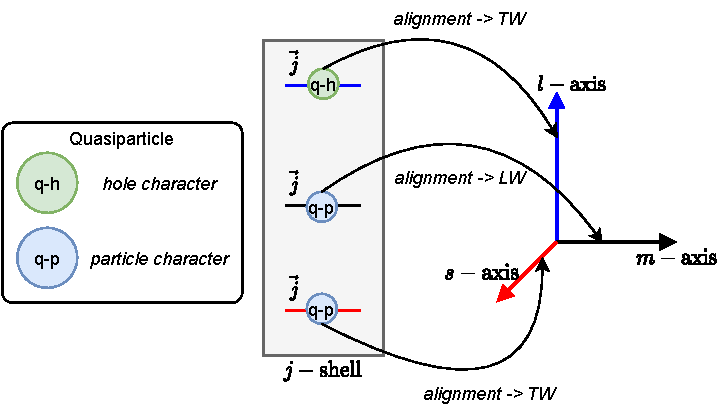
\includegraphics[width=0.95\textwidth]{figs/wobbling_Regimes.pdf}
    \caption{The wobbling regime (LW or TW) based on the type of alignment for an odd quasiparticle with the triaxial core. Figure based on the quantal analysis done in \cite{frauendorf2014transverse}.}
    \label{quasiparticle-alignment}
\end{figure}

As previously mentioned, for a given angular momentum, uniform rotation around the axis with the largest MOI corresponds to a minimum energy. For a triaxial rotor, this is equivalent to rotation around the $m$ axis. Therefore, Frauendorf \cite{frauendorf2014transverse} classified the LW as the situation when the odd nucleon will align its angular momentum along the $m$-axis, while TW being the situation where $j$ is aligned perpendicular to the $m$-axis (with $s$- or $l$-axis alignment depending on the $j$-shell orbital from which the odd nucleon arises). It is worthwhile to mention the fact that the analysis done in Ref. \cite{frauendorf2014transverse} was within a so-called \emph{Frozen Alignment} approximation, where the angular momentum of the odd particle $\vec{j}$ is rigidly aligned with one of the three principal axes of the triaxial ellipsoid (that is $s$-, $l$- or $m$-axis).

For a better understanding of the wobbling regimes in terms of angular momentum alignment, the schematic illustration from Figure \ref{wobbling-coupling-scheme} depicts three particular cases, namely a simple wobbler (the case firstly developed by Bohr and Mottelson \cite{bohr1998nuclear}) - shown in inset A.0, a longitudinal wobbler - shown in inset A.1, and lastly a transverse wobbler - shown in inset A.1.

\begin{figure}
    \centering
    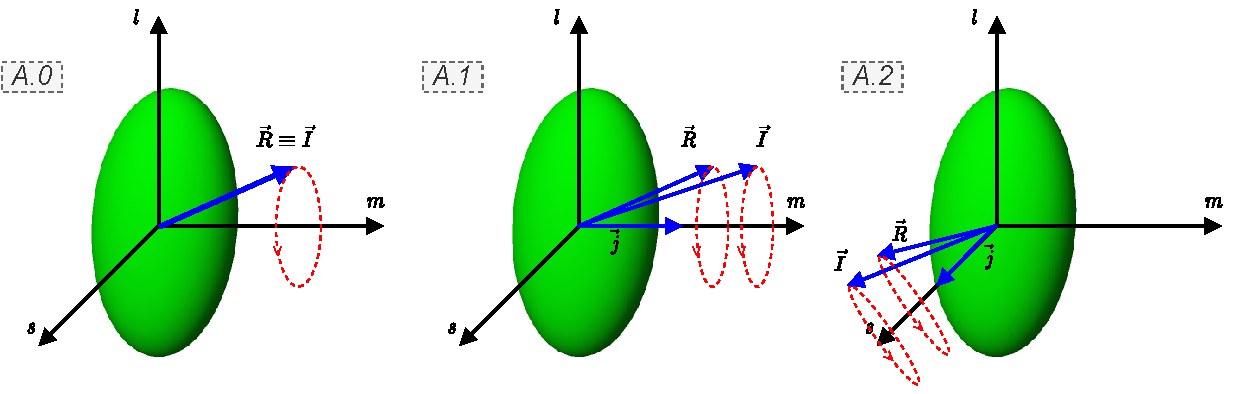
\includegraphics[width=0.95\textwidth]{figs/wobbling_Regimes_COUPLING_SCHEME.pdf}
    \caption{The geometry for the angular momentum for a simple wobbler: A.0, a longitudinal wobbler: A.1, and a transverse wobbler: A.2. The short, long, and medium axes are defined in the body-fixed frame. The vectors $\vec{R}$, $\vec{j}$, and $\vec{I}$ represent the set of angular momenta of the core, odd particle, and the total nuclear system, respectively.}
    \label{wobbling-coupling-scheme}
\end{figure}

In terms of its theoretical analysis, the wobbling motion has been studied using multiple models and interpretations. The Triaxial Particle Rotor Model has been widely used over the recent years \cite{bohr1998nuclear,hamamoto2002wobbling,frauendorf2014transverse,tanabe2006algebraic,wen2015wobbling}, these being quantal models that can be exactly solved in the laboratory frame. TRM was however, firstly introduced for the motion of a rotating nuclear system by Davydov and Filippov in \cite{davydov1958rotational}, where they obtained a complete quantal description for the motion of a triaxial nucleus (considering the fact that the nucleus must have a well-defined potential minimum at a non-zero value for the triaxiality parameter $\gamma$). Starting from the framework of Cranking Mean Field Theory (CMFT), there were attempts at extending the cranking model for the study of WM. however, using the mean field approximations, CMFT only help at describing the yrast sequence for a given configuration. In order to improve that, the framework was extended with proper quantum correlations by incorporating the Random Phase Approximation (RPA) theory (see Refs. \cite{shimizu1995nuclear,matsuzaki2002wobbling,matsuzaki2003dynamical,matsuzaki2004instability,matsuzaki2004nuclear,shimizu2005high,shimizu2008parametrizations,shoji2009microscopic} for more details).  The method of Collective Hamiltonian \cite{chen2014collective,chen2016wobbling} was used for the investigation of wobbling spectra in nuclei with the help of deformed potentials which were calculated from the Tilted Axis Cranking (TAC) model. TAC single $j$-shell model is also used for the description of the chiral vibrations and rotational motion in deformed nuclei \cite{mukhopadhyay2007chiral,qi2009chirality}. Mean field approximations were also developed by the so-called \emph{generator coordinate method after angular momentum projection} (GCM+AMP for short), with calculations that emerged from intrinsic cranking states \cite{oi2000wobbling}. Some analytical solutions were also developed (based on certain approximations), such as the harmonic approximation (HA) \cite{bohr1998nuclear,frauendorf2014transverse,chen2014collective,raduta2017semiclassical}, Dyson boson expansion \cite{raduta2017semiclassical,raduta2020new}, and Holstein-Primakoff (HP) formula \cite{tanabe1971triaxiality,tanabe2006algebraic,tanabe2008selection,raduta2017semiclassical,raduta2020new}. The angular momentum projections were also incorporated into the mean field framework, with the recent development of a completely microscopic description of the wobbling motion by Shimada et. al. \cite{shimada2018rotational}. A Projected Shell Model (PSM) \cite{hara1995projected} which starts from the shell-model configuration mixing that is based on a Nilsson deformed mean field was also used for the theoretical study concerning WM. There are alternative developments based on the PSM approach, based on Density Functional Theories (DFT) that can be both non-relativistic \cite{zhao2016configuration} as well as relativistic \cite{konieczka2018gamow}.

Other tools that proved to be very efficient for the analysis of the wobbling nuclei are the semi-classical approaches, through which one can obtain equations of motion that describe the nuclear system quite well, starting from quantal Hamiltonians and further applying some de-quantization procedures. The semi-classical approach applied to generalized rotor Hamiltonians has the \emph{advantage} of keeping close contact with the classical picture embedded in the dynamic of the systems. Recently, there has been quite an impressive progress towards realistic description of the wobbling motion \cite{raduta2007semiclassical,frauendorf2014transverse,raduta2017semiclassical,raduta2018wobbling,budaca2018tilted,raduta2020approach,raduta2020towards}. As a matter of fact, the present team was able to describe (with a very good agreement) the experimental data concerning the wobbling energies and electromagnetic (e.m.) transition probabilities for the Lu isotopes with $A=161,163,165,167$ (see the work done in Refs. \cite{raduta2017semiclassical,raduta2018wobbling}), and more recently the odd-$A$ $^{135}$Pr isotope \cite{raduta2020new}. Indeed, starting from a quantal Hamiltonian specific to a triaxial rotor model (that is a triaxial core coupled with an odd valence nucleon) and applying the Time Dependent Variational Equation (TDVE), with a trial function that was carefully chosen, the complete wobbling spectrum of the mentioned isotopes was reproduced, together with the e.m. (intra-band and inter-band) transitions.

Concluding this section, the importance of nuclear triaxiality and the challenges of identifying it experimentally were contoured in the beginning, serving as the starting point of the current work. Furthermore, all the known nuclei in which wobbling motion appears were mentioned (with important observation for some of them). Additionally, the mechanism behind the simple wobbler (the one developed by Bohr and Mottelson \cite{bohr1998nuclear}) was sketched (starting with Eq. \ref{wobbling_eq}), and a family of wobbling bands were schematically represented for a given set MOIs associated to the triaxial rotor (see Figure \ref{simple-wobbling-family}). Lastly, a brief overview with most of the theoretical \emph{tools} that were/are used for describing this elusive phenomenon was realized. Having this in mind, one can say that a detailed outlook for the topic of wobbling motion was properly shown.

Going further, the remaining structure of this current work must be pointed out. In Section 2, an overview with regards to the team's reinterpretation of the wobbling band structure in $^{163}$Lu will be illustrated. This will be the \emph{core-idea} that serves as foundation of this newly developed model. The theoretical formalisms and analytical formulas will be properly presented in Section 3. Experimental results concerning the wobbling spectrum of this isotope will be compared with the newly obtained data in Section 4. Overall conclusions and discussions are reserved to Section 5. 

\section{Re-interpretation of the wobbling bands structure for $^{163}$Lu}

Now that a complete overview of the recent experimental and theoretical results regarding wobbling motion has been made, together with the description of its two regimes (namely, longitudinal wobbling and transverse wobbling), it is worth mentioning the latest progress made by the present team towards the actual interpretation of the wobbling structure of $^{163}$Lu. Considered the \emph{best wobbler} to date, $^{163}$Lu has a rich wobbling spectrum \cite{odegaard2001evidence,jensen2002evidence}, with no less than four such wobbling bands: one yrast - $TSD_1$, which has a zero-phonon wobbling number $n_w=0$), and three excited wobbling bands - $TSD_{2,3,4}$ with their corresponding wobbling phonon numbers $n_w=1,2,3$, respectively. The name TSD comes from Triaxial Strongly Deformed bands. The triaxial bands emerge due to the coupling of an odd-$\vec{j}$ nucleon with an even-even triaxial core. Thus, for $^{163}$Lu, it is the intruder $\pi(i_{13/2})$ that couples to the triaxial core \cite{odegaard2001evidence,hamamoto2002wobbling,jensen2002wobbling}, driving the nuclear system up to large deformation, and stabilizing the deformed structure. Indeed, a triaxial shape with deformation parameters $(\epsilon_2,\gamma)\approx(0.38,+20^\text{o})$ is assumed to be in agreement with the observed data, based on calculations using the Ultimate Cranker Code \cite{bengtsson1990high} for the potential energy surface (PES).

In terms of experimental evidence which should be pointing out wobbling nature for the four TSD bands belonging to $^{163}$Lu, the large transition quadrupole moment $Q_t \approx 10\ b$ \cite{gorgen2004quadrupole} (which is substantially larger than it is the case for normal-deformed bands), the predominantly $E2$ character of the transitions linking adjacent bands ($I\to I-1$), a large $E2/M1$ mixing ratio $\delta>1$ for the transitions linking the yrare ($n_w=1$) and yrast ($n_w=0$) bands (which obviously should result in smaller transitions with magnetic character, or in other words, there is no $M1$ dominance) are clear fingerprints of wobbling nature. For a set of results concerning these quantities (both theoretical and experimental), see Ref. \cite{raduta2017semiclassical}, and the references cited therein. Another quantity that indicate strong deformation with wobbling character is the relative rigid rotor energy, and for this isotope calculations show that all four bands have a similar behavior with respect to this value (see Figures 3 and 4 from Ref. \cite{hagemann2005triaxiality}).

Considering the experimental evidence which was indicated above and calculations based on particle rotor models, it can be summarized that the \emph{generally accepted} formalism for the band structure in $^{163}$Lu is the following:
\begin{itemize}
    \item There are three excited wobbling bands (w.b.): $TSD_2$, $TSD_3$, and $TSD4_4$.
    \item The three excited w.b. have wobbling-phonon numbers $n_{w_2}=1$, $n_{w_3}=2$, and $n_{w_4}=3$, respectively.
    \item All three bands are built on top of the yrast state (the ground state band) with zero-wobbling-phonon number $n_{w_1}=0$.
    \item Stable triaxial super-deformation is achieved due to the alignment of the odd $\pi(i_{13/2})$ nucleon which couples to a triaxially deformed core $\vec{R}$.
    \item $TSD_{1,2,3}$ have all positive parity $\pi_1=\pi_2=\pi_3=+1$, while the spin states belonging to $TSD_4$ have negative parity $\pi_4=-1$. All states within the four bands have half-integer spin, obviously.
 \end{itemize}

In accordance with the band structure which was just formulated, a full description of the wobbling spectrum of $^{163}$Lu was done within a semi-classical formalism by Raduta et. al. \cite{raduta2017semiclassical}. Therein, with the TDVE applied on the PRM Hamiltonian with a trial wave-function that encapsulates both the states of the deformed nucleus $I$ and the single-particle states $j$, a set of analytical expressions for the excitation energies of all four bands was obtained. The energies belonging to the excited wobbling phonons were populated by the action of a phonon operator $\Gamma^\dagger$ on the ground state. Indeed, by acting with the operator one on the ground state with the spin $I=R+j$ and $R=0,2,4,\dots$, the states from $TSD_2$ ($n_w=1$) can be obtained. By applying twice ($n_w=2$) the phonon operator, the rotational states from $TSD_3$ will be created. Lastly, the states from $TSD_4$ are obtained with the action on the ground state with three ($n_w=3$) phonon operators: two of positive parity and one of negative parity (due to the overall negative parity $\pi_4=-1$ of $TSD_4$). One has to remark the fact that for $TSD_4$, the model assumes an odd-particle-rotor with a different intruder: the $\pi(h_{9/2})$ nucleon. This was suggested by the negative parity orbital which might be occupied by this proton, in the spherical shell model. Several calculations in the literature point out that this nucleon might be causing the third excited wobbling band to have negative parity \cite{jensen2004coexisting}. It is worthwhile mentioning that for the work described in \cite{raduta2017semiclassical}, the variational principle was only applied for the states in $TSD_1$, since the other three wobbling bands are obtained through phononic excitations with the corresponding operator.

In what follows, it is useful to introduce some notations that will refer to the formalisms developed by the team in describing the wobbling motion in $^{163}$Lu. As such, the work developed in \cite{raduta2020approach,raduta2020towards} will be denoted to \texttt{W1}, while the current work (which is in fact an extension of \texttt{W1}) will be shortly denoted by \texttt{W2}. For the sake of a self-consistent presentation, in the following subsection \ref{subsection:w1} a brief overview of the recently published work \texttt{W1} will be made, with further development that has \texttt{W1} as a starting ground being presented in the second subsection \ref{subsection:w2} - representing the \emph{core concept} of the current team's investigation.

\subsection{\texttt{W1} - Signature Partner Bands}
\label{subsection:w1}

Working with a semi-classical approach that is based on the triaxial particle rotor model, a full description of the wobbling bands for $^{163}$Lu was achieved, but with a slightly modified band structure. Indeed, rather than applying a TDVE just for the yrast $TSD_1$ band, the states from $TSD_2$ were also obtained variationally. This was possible due to the different coupling schemes that emerged for $TSD_1$ and $TSD_2$, respectively. More precisely, in \cite{raduta2020towards} and \cite{raduta2020approach} there are three different coupling schemes $(\vec{R}+\vec{j})$: states from $TSD_1$ arise from the odd $\pi(i_{13/2})$ intruder coupling with a core with angular momentum sequence $R_1=0,2,4,\dots$; states from $TSD_2$ arise from the same odd proton but coupling with a different triaxial core with angular momentum sequence $R_2=1,3,5,\dots$. The band $TSD_3$ is obtained as a set of states which are built on top of $TSD_2$, with the action of a wobbling frequency with wobbling phonon number $n_w=1$; this being different than the band structure previously mentioned where the third band was a two-phonon excitation of the yrast $TSD_1$. Lastly, the fourth band $TSD_4$ is a ground state band which results from the coupling of the same core as for $TSD_2$ (that is defined with the angular momentum sequence $R_2=1,3,5,\dots$) but with a different odd nucleon: $\pi(h_{9/2})$. Consequently, $TSD_2$ and $TSD_4$ are yrast states, alongside $TSD_1$. Each band represents a collection of energy levels describing ground states that correspond to distinct sets of angular momenta.

For the first three bands, the MOIs are the same, and they are considered to be free parameters within the numerical calculations. However, this is not true for the fourth band, where a different set of MOIs had to be introduced, since for $TSD_4$ the core polarization effects are changed by coupling scheme.

Using \texttt{W1}, the final results pointed out to a largest MOI corresponding to the 1-axis (with $\mathcal{I}_1$ being the largest MOI obtained through the fitting procedure), making the system rotate around the 1-axis (that is the short axis). Moreover, the odd proton is aligned to the short axis as well, suggesting that the nucleus has a LW character. By representing the experimental wobbling energies according to Eq. \ref{wobbling-energy-relative}, it was obtained that both theoretical as well as the experimental values were increasing functions with respect to an increase in angular momentum (keep in mind that the first wobbling band $n_w=1$ within the \texttt{W1} model is $TSD_3$). The agreement between the two sets of data (see Figure 6 from \cite{raduta2020approach}) indicate that the condition for LW/TW character of the wobbling bands stated by Frauendorf et. al. in \cite{frauendorf2014transverse} is not strictly related to the increasing/decreasing wobbling energy $E_\text{wob}$. In fact, Guo et. al. \cite{guo2020risk} also point out that the approximation of Frozen Alignment (FA) from \cite{frauendorf2014transverse} neglects the Coriolis interaction of the single particle. There is an ongoing debate whether the behavior of an LW or TW triaxial nucleus is strictly related to the change in $E_{wob}$ with total a.m. \cite{tanabe2017stability,frauendorf2018comment,tanabe2018reply}.


A final aspect that needs to be mentioned regarding \texttt{W1} has to do with the interpretation of $TSD_1$ and $TSD_2$ as being Signature Partner Bands (SPB). Signature is a quantum property strictly related to the invariance of the nuclear wave-function to a rotation by an angle $\pi$ around an axis that is perpendicular to the symmetry axis. Because the triaxial rotor Hamiltonian has a $D_2$ symmetry property, signature quantum number is a good quantum number for the case of non-axially symmetric nuclei. In \cite{raduta2020approach} the signature concept is brought to the classical picture associated to a triaxial nucleus by means of rotation operators which act on the trial function (this function is a product of two coherent states, one that is associated to the core and one to the valence nucleon). Eqs. 27-29 from \cite{raduta2020approach} will extract two signatures for $TSD_1$ and $TSD_2$, namely the \emph{favored} signature $\alpha_{1f}=+1/2$ for the first band, and \emph{un-favored} signature $\alpha_{2u}=-1/2$ for the second band, respectively. A justification for the possibility of $TSD_1$ and $TSD_2$ of being SPB was based on the calculation of the triaxial potential (which was systematically performed in \cite{raduta2017semiclassical} and \cite{raduta2018wobbling}), concluding that the minimum is very deep, preventing in this way the states from $TSD_2$ to share other minima through tunneling effects.

A few key-points which arise based on the above discussion regarding \texttt{W1} can be summarized as follows:

\begin{enumerate}[(a)]
    \item The wobbling band structure in $^{163}$Lu was re-interpreted: three bands are now yrast ground states, and only $TSD_3$ is one-phonon excited wobbling band (built on top of $TSD_2$)
    \item Both $TSD_1$ and $TSD_2$ are obtained variationally, by solving the time dependent variational equation associated to the initial quantal Hamiltonian
    \item There are three different $R+j$ coupling schemes that will produce the entire spectra:
    \begin{enumerate}[(i)]
        \item Coupling $C_1$: The odd proton $j_1={13/2}$ is coupled to a core sequence with a.m. $R_1=0,2,4,\dots$ (even spin states for the triaxial rotor).
        \item Coupling $C_2$: The same odd proton $j_1={13/2}$ as in $C_1$ is coupled to a core sequence with a.m. $R_2=1,3,5,\dots$ (odd spin states for the triaxial rotor).
        \item Coupling $C_3$: A different odd proton $j_2={9/2}$ is coupled to the same core as in $C_2$.
    \end{enumerate}
    \item Two different sets of MOIs corresponding to the triaxial nucleus (that is the rotor coupled with the odd proton) are obtained as fitting parameters throughout the numerical calculations: one for the set $TSD_{1,2,3}$ and one for for $TSD_4$.
    \item $TSD_1$ and $TSD_2$ are Signature Partner Bands: with $TSD_1$ ($TSD_2$) being the favored (un-favored) partner. Their corresponding signature quantum numbers are $\alpha_{1f}=+1/2$ and $\alpha_{2u}=-1/2$.
    \item As a side-by-side comparison with regards to the overall agreement with the experimental data, \texttt{W1} yielded better results than compared to the previous work depicted in Ref. \cite{raduta2007semiclassical}, although it must be mentioned that both models are based on semi-classical approaches.
\end{enumerate}

A diagram which shows the workflow involved in \texttt{W1} can be seen in the Figure \ref{w1-model-worfklow}. Also, a comparison with previous calculations can be seen in Figure 21 from Ref. \cite{raduta2020approach}.

\begin{figure}
    \centering
    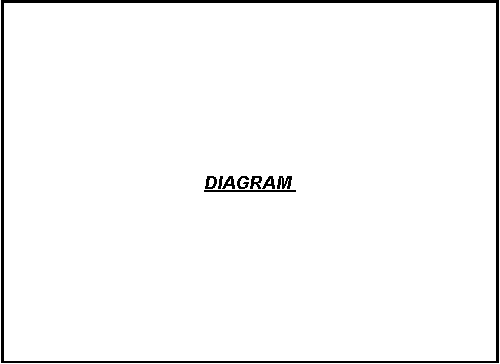
\includegraphics[scale=0.65]{figs/W1_W2_models.pdf}
    \caption{The general workflow involving \texttt{W1} model.}
    \label{w1-model-worfklow}
\end{figure}

\subsection{\texttt{W2} - Signature Partner Bands + Parity Partner Bands}
\label{subsection:w2}

The main question which can be asked regarding the formalism \texttt{W1} that was described in \ref{subsection:w1} is whether it is possible to obtain a \emph{unified} description for all four bands in $^{163}$Lu in relation to the coupling scheme. In other words, it is worth investigating the possibility of having an unique single-particle state $j$ that is coupled to a core of natural positive parity (hereafter denoted by $R_1$) for the bands $TSD_{1,2,3}$ and a core of negative parity for $TSD_4$ (hereafter denoted by $R_2$).

Fortunately, the answer is positive: starting from the semi-classical formalism of \texttt{W1}, one can properly adjust the coupling scheme, making sure that the entire numerical recipe used for obtaining the energy spectrum of $^{163}$Lu remains consistent with the experimental results.

Regarding the unique single-particle that couples to the triaxial core, it is natural to pick the $i_{13/2}$ proton (that is $j_1$ from \texttt{W1}). Reasoning behind this choice has to do with the microscopic calculations \cite{jensen2002wobbling,hagemann2003quantized,jensen2004coexisting} that showed stable triaxial structures in the $^{163}$Lu potential energy surface when the triaxial core couples with a highly aligned $j$-shell particle, strongly indicating the $\pi(i_{13/2})$ proton.

By taking $j_1$ as the sole intruder that couples to a positive core ($R_1$) and also a negative core ($R_2$), the even/odd spin sequences for the coupling schemes does not change. In fact, the coupling schemes can be readily obtain, making sure that the final (experimental) spin sequences for each TSD band is intact. 

\begin{enumerate}[(a)]
    \item Coupling $C'_1$: the odd $j_1$ proton aligns with the core of even-integer spin sequence $R_1=0,2,4,\dots$, with a parity of the $R_1$ core that is positive $\pi_1=+1$.
    \item Coupling $C'_2$: the odd $j_1$ proton aligns with the core of even-integer spin sequence $R_2=1,3,5,\dots$, with a parity of the $R_1$ core that is positive $\pi_1=+1$.
    \item Coupling $C'_3$: the odd $j_1$ proton aligns with the core with an odd-integer spin sequence $R_1=1,3,5,\dots$, which has negative parity $\pi_2=-1$.
\end{enumerate}

From the three schemes sketched above, it is clear that $C'_1$ corresponds to the yrast $TSD_1$, $C'_2$ to the ground state $TSD_2$, and finally $C'_3$ to the ground state $TSD_4$. Obviously, the odd valence nucleon $j_1$ has a positive parity $\pi_{j_1}=+1$. 

Concluding the current subsection, a diagram which shows the workflow involved in \texttt{W2} can be seen in the Figure \ref{w2-model-worfklow}.

\begin{figure}
    \centering
    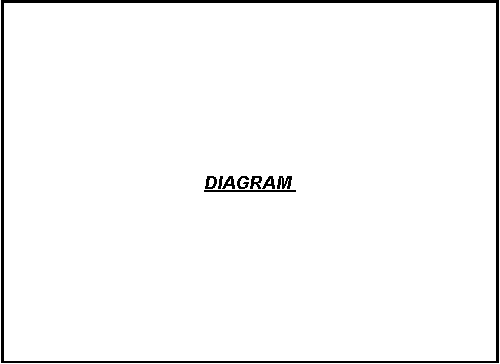
\includegraphics[scale=0.65]{figs/W1_W2_models.pdf}
    \caption{The general workflow involving \texttt{W2} model.}
    \label{w2-model-worfklow}
\end{figure}

\section{Theoretical Background}

The Hamiltonian of the system is given in terms of a term that corresponds to the core deformation, and a second term which corresponds to the valence nucleon moving in a mean-field with quadrupole character (generated by the triaxial core).

\begin{align}
    \hat{H}=\hat{H}_\text{rot}+\hat{H}_\text{s.p.}.
\end{align}

%%%%%%%%%%%%%%%%%%%%%%%%%%%%%%% TEXT  %%%%%%%%%%%%%%%%%%%%%%%%%%%%%%%%%%%%%%%%%

\bibliography{dev-refs}

\end{document}  